\documentclass{hw}
\hwname{6 / Radicals / WP-1}

\begin{document}

\subsection*{\normalsize Gravitation Force problem}
Some laws of nature have squares - especially for the distance terms.

\subsubsection*{\normalsize Problem Statement}

\begin{figure}[h]
    \centering
    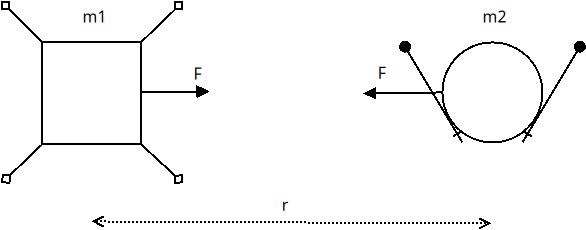
\includegraphics[width=0.6\textwidth]{dia/radicals-satellites.png}
    \caption{Two satellites in space.}
    \label{fig:satellites}
\end{figure}

Two space satellites, each with a mass of 100 kg, are observed to attract each other with a gravitational force of 25 Newtons.\\
The force follows the equation:

{\centering
$F = G \frac{m_1 m_2}{r^2}$
\par}

where,
\begin{itemize}
    \item $m_1$ and $m_2$ are the masses of the two objects in kilograms
    \item $r$ is the distance between the objects in meters
    \item $G$, the gravitational constant, is equal to 1 (in this simplified universe)
    \item $F$ is the gravitational force between the two objects in Newtons 
\end{itemize}
\bigskip
What is the distance between the two satellites?

\subsubsection*{\normalsize Solution}

%\begin{align*}
%25 &= \frac{1 \times 100 \times 100}{r^2} \\
%r^2 &= \frac{10000}{25} \\
%r^2 &= 400 \\
%r &= 20
%\end{align*}
%The distance between the two satellites is 20 meters.

\end{document}